% ---------------------------------------------------------------------------------------------
% Section 3: Method and Progress (#15). Paste after Section 2 (Related Work), before References.
% Needs \usepackage{tikz} (already used by Figure 1) and booktabs (loaded by acmart).
% Citation keys: rename to match the project's .bib if they differ (see README.md in this folder).
% ---------------------------------------------------------------------------------------------

\section{Method and Progress}
\label{sec:method}

Our project is an empirical study whose instrument is a tool. This section describes the
components we have built, how we check that they measure what we claim, what the first agent
runs show, and what remains. Everything described here is in a public repository with
continuous integration,\footnote{\url{https://github.com/Yash-11-star/religuard}. Version~0 is tag
\texttt{v0}; the results below are under \texttt{results/} (\texttt{v0/}, \texttt{mutants/},
\texttt{pilot/}).} and every number below can be reproduced with the scripts in it.

\subsection{Changes since the proposal}
\label{sec:scope}

We made one scope change. The proposal ran the subject system on Kubernetes (Kind) with
Chaos Mesh~\cite{chaosmesh}. For the midpoint we built it on docker-compose instead and inject
all faults with Toxiproxy~\cite{toxiproxy}. Every fault our properties need (added latency,
an unreachable service, responses lost after the server acted) is a network fault that Toxiproxy
produces directly, and docker-compose let us reach a stable baseline and a first agent run in
the time available. Moving to Kind and adding Chaos Mesh for pod-level faults (container kills,
restarts) is the first milestone after the midpoint (Section~\ref{sec:remaining}). The research
questions, the three agents, the eight changes, and the 72-version design are unchanged.

\subsection{Subject system: Version 0}
\label{sec:v0}

Version~0 is a checkout service built from three Python (FastAPI) services and a PostgreSQL
database (Figure~\ref{fig:arch}). \emph{Order} receives \texttt{POST /checkout}, reserves stock in
\emph{Inventory}, charges the customer through \emph{Payment}, and then commits or releases the
reservation. Every call from Order to its dependencies, including to its own database, passes
through Toxiproxy, so a test can slow down, cut off, or silence any dependency without changing
any code. Payment and Inventory also expose small \texttt{/admin} endpoints that let a check count
charges and attempts, read stock levels, and force HTTP 503s or card declines, which Toxiproxy
cannot produce.

We wrote Version~0 to be correct under failure, using the patterns that the retry-bug study of
Stoica et al.~\cite{stoica2024retry} identifies as commonly gotten wrong:
(i)~a 1\,s timeout on every attempt and a 2.5\,s deadline for the whole checkout, so a slow
dependency cannot make checkout hang;
(ii)~at most three attempts with jittered exponential backoff, retrying only timeouts, connection
errors, and 502/503/504;
(iii)~the same idempotency key (\texttt{order-<id>}) on every charge attempt, and an idempotency key
on the checkout request itself, so neither retries nor duplicate deliveries charge twice;
(iv)~compensation: a failed or abandoned checkout releases its stock reservation, and a background
task finishes or fails every order, so none stays \texttt{PENDING}; and
(v)~a 1\,s bound on each database statement.
These mechanisms are exactly what an agent can quietly remove while adding a feature.

\begin{figure}[t]
  \centering
  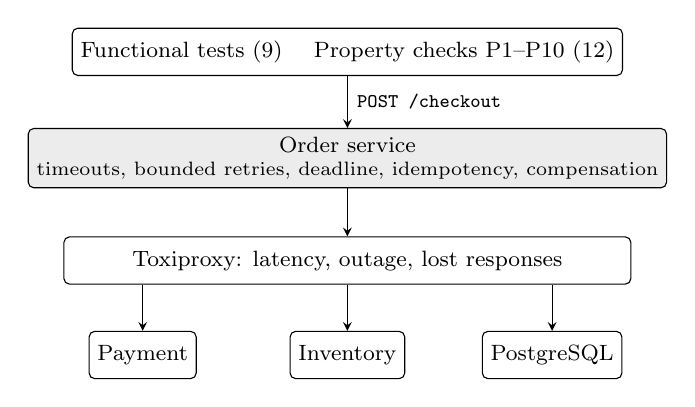
\begin{tikzpicture}[font=\footnotesize, >=stealth,
      box/.style={draw, rounded corners=2pt, align=center, inner sep=3pt, minimum height=0.6cm}]
    \node[box] (checks) at (0,2.5) {Functional tests (9) \quad Property checks P1--P10 (12)};
    \node[box, fill=gray!15] (order) at (0,1.15) {Order service\\[-1pt]
      \scriptsize timeouts, bounded retries, deadline, idempotency, compensation};
    \node[box, minimum width=7.2cm] (tox) at (0,-0.15) {Toxiproxy: latency, outage, lost responses};
    \node[box] (pay) at (-2.6,-1.35) {Payment};
    \node[box] (inv) at (0,-1.35) {Inventory};
    \node[box] (db) at (2.6,-1.35) {PostgreSQL};
    \draw[->] (checks) -- node[right, font=\scriptsize] {\texttt{POST /checkout}} (order);
    \draw[->] (order) -- (tox);
    \draw[->] (tox.south -| pay) -- (pay);
    \draw[->] (tox) -- (inv);
    \draw[->] (tox.south -| db) -- (db);
  \end{tikzpicture}
  \caption{Version~0. The checks drive checkout over HTTP, inject faults through Toxiproxy's API,
  and read the outcome from the services' \texttt{/admin} endpoints.}
  \label{fig:arch}
\end{figure}

\subsection{Reliability properties as executable checks}
\label{sec:props}

Following design choice D1, we wrote the ten reliability properties as pytest checks before any
agent touched the code (Table~\ref{tab:props}). Each check pairs one fault with one expected
behavior, starts and ends with every fault removed and every table cleared, and judges only what
a client or an operator could observe: the response, its latency, the number of charges and
attempts Payment recorded, stock levels, and order states. None of them depends on how Order is
implemented, so they remain valid after an agent restructures the code. P6 and P8 each run two
cases, giving 12 test cases. Separately, nine \emph{functional} tests check the store without
any fault (successful checkout, lookup, out-of-stock, invalid input, repeated request, declined
card). They play the role of the tests an agent normally relies on, and RQ1 compares the two pass
rates.

\begin{table*}[t]
  \caption{Reliability properties. \emph{Version~0} is the value we measure on the baseline.}
  \label{tab:props}
  \small
  \begin{tabular}{@{}l p{5.4cm} p{6.6cm} l@{}}
    \toprule
    & Fault injected & Expected behavior & Version 0 \\
    \midrule
    P1  & Payment responses delayed 5\,s & Checkout returns an error within 3\,s & 504 in 2.5\,s \\
    P2  & Inventory responses delayed 5\,s & Checkout returns an error within 3\,s & 504 in 2.5\,s \\
    P3  & Payment unreachable & HTTP 503 with a JSON error body within 3\,s & 503 in 0.3\,s \\
    P4  & Payment returns 503 to the next 10 calls & Payment receives at most 3 attempts for the checkout & 3 attempts \\
    P5  & Payment charges, but its responses are lost; client retries with the same key & Exactly one charge & 1 charge \\
    P6  & Same checkout sent twice (sequentially; concurrently) & One order, one charge, same order returned both times & 1 order, 1 charge \\
    P7  & Payment unreachable, then restored & A new checkout succeeds within 10\,s of the restore & 0.5\,s \\
    P8  & Payment declines; Payment unreachable & Reserved stock is returned within 5\,s & Released \\
    P9  & One checkout under each of 7 faults above & No order left \texttt{PENDING} 5\,s after faults are removed & None left \\
    P10 & Each orders-DB round trip delayed 1.5\,s & 503/504 JSON error within 3\,s; healthy after & 503 in 1.0\,s \\
    \bottomrule
  \end{tabular}
\end{table*}

\paragraph{Is the oracle trustworthy?}
Our definition of a regression (a property that passed on the previous version and fails on the
next) is only as good as the checks. We validated them in three ways.
\emph{Stability:} on Version~0, five consecutive runs from a clean reset passed 9/9 functional
tests and 12/12 property checks every time (about 26\,s per run), so a failure is not noise.
\emph{Sensitivity:} we planted six faults of the kind an agent might introduce into Order, in the
spirit of mutation analysis~\cite{jia2011mutation}. The checks caught five: raising the retry cap
to 6 (P4), removing timeouts (P1, P2, P9), using a fresh idempotency key on each retry (P5),
never releasing stock (P8), and removing the task that finishes stale orders (P9). The sixth,
raising the database timeout to 10\,s, was not observable: the 2.5\,s checkout deadline still
bounded the response. The behavior was still correct, so we treat it as an equivalent mutant,
not a missed regression. The nine functional tests, by contrast, caught only one of the six (never
releasing stock, through the declined-card test), which previews the gap RQ1 measures.
\emph{The pilot itself:} the first agent run exposed two checks that asserted the wrong thing
(Section~\ref{sec:pilot}); we fixed both and re-measured.

\subsection{Change sequence and agent harness}
\label{sec:harness}

We wrote the eight change requests as ordinary product tickets: a notification service, more
payment retries, a stock cache, per-customer rate limiting, notifications through a message queue,
an order history table, an order-cancel endpoint with refund and restock, and a longer payment
timeout. None mentions reliability, faults, or the properties. Several are deliberately tempting
(``retry payment more'', ``raise the timeout''), because that is how real reliability regressions
are introduced.

The harness keeps runs comparable and keeps the oracle hidden. For each run it exports Version~0
into a fresh repository and removes the property checks, the study materials, and every mention of
them (in code comments, the README, and CI), then confirms with a keyword search that nothing
remains. The agent sees a normal repository with its own tests, as a real team's would be.
For change~$i$, the harness gives the agent a fixed preamble plus change request~$i$, runs it once
headless with a pinned model and no follow-up messages, and commits whatever it produced. It then
starts the agent's version of the stack, runs the agent's own tests, and runs the full property
suite from outside the workspace (design choice D2). Every value each check measured is recorded
(latencies, status codes, attempt and charge counts, stock), not only pass or fail. Any failing
check is re-run once on its own: a check that fails both times counts as a regression, and one
that passes on the re-run is marked flaky. The next change starts from this version, so mistakes
can accumulate.

\subsection{Progress: first agent results}
\label{sec:pilot}

We piloted the full pipeline with Claude Code (CLI 2.1.309, model \texttt{claude-sonnet-5-5}) on
the first two changes (Table~\ref{tab:pilot}). Both changes completed without help, and the agent's
own tests passed every time. Change~01 added a Notification service (11 files, +311/$-$22 lines)
and broke no property. Change~02, ``retry payment more on transient failures'' (3 files,
+91/$-$22 lines), broke three. The agent replaced
the cap of three attempts with up to 30 attempts inside a separate 20\,s retry window that no longer
respected the checkout deadline. Under ten 503s, Payment now received 11 attempts (P4). With Payment
slow or unreachable, checkout answered after 18--20\,s instead of within 3\,s (P1, P3). The agent
also rewrote the existing test that asserted ``answers within 3\,s'' so that it expected a 504
after the retry window, which is why its 47 tests all passed. In other words, the agent changed the
test to match the regression. This is the effect our study is designed to measure: an agent that
completes a ticket correctly by every check it can see, while removing a guarantee no one asked it
to remove.

\begin{table}[t]
  \caption{Pilot: Claude Code, run 1. ``Own tests'' are the tests in the agent's repository,
  including any it added or changed.}
  \label{tab:pilot}
  \small
  \begin{tabular}{@{}l r r l@{}}
    \toprule
    Version & Agent time & Own tests & Properties \\
    \midrule
    Version 0       & --     & 30/30 & 12/12 \\
    01 Notification & 84\,s  & 43/43 & 12/12 \\
    02 Retries      & 104\,s & 47/47 & 9/12 (P1, P3, P4) \\
    \bottomrule
  \end{tabular}
\end{table}

The pilot also tested our method, and found three problems with it. First, two checks asserted
``checkout failed'' before measuring their property, so when change~02 made checkout succeed after
many retries, P4 stopped before counting attempts and P8 failed although stock was handled
correctly. We changed P4 to measure first and P8 to take Payment down for the whole checkout,
which no retry policy can outlast. We then re-measured Version~0 (still 12/12) and change~02
(the same three regressions, now with the attempt count recorded). Second, the agent's output
format saved only its final message; the study runs will record the full turn-by-turn transcript,
which RQ2's root-cause analysis needs. Third, the properties never exercise a dependency that an
agent adds, such as change~01's Notification service (Section~\ref{sec:challenges}).

\subsection{Remaining work}
\label{sec:remaining}

\begin{itemize}
  \item \textbf{Week 1:} move the stack to Kind with Chaos Mesh for pod-level faults; add request
  tracing for the evidence in D3; turn the pilot scripts into one harness command with adapters
  for Claude Code, Codex CLI, and Copilot's coding agent, which resumes after interruptions.
  \item \textbf{Week 2:} build \textsc{ReliGuard}'s evidence builder (fault, expected property, measured
  values, trace, and the diff hunk that introduced the change) and the repair loop that accepts a
  fix only if the entire suite passes (D4); make all three agents run headless.
  \item \textbf{Week 3:} the main study (3 agents $\times$ 3 runs $\times$ 8 changes = 72 versions)
  and the repair experiment.
  \item \textbf{Week 4:} analysis for RQ1--RQ3, manual root-cause categorization, and figures,
  followed by the final report and public release of the benchmark.
\end{itemize}

\subsection{Challenges}
\label{sec:challenges}

\textbf{Requested versus collateral regressions.} Change~02 asked for more retries, so is 11 attempts
a regression or the feature? The request never asked to give up the 3\,s response bound, and
the agent could have retried more within the deadline. We will still label each regression as
\emph{collateral} (a property the request did not touch) or \emph{in tension} with the request,
and report both, so readers can apply the stricter definition.

\textbf{Properties do not cover what agents add.} Our checks exercise the dependencies of Version~0.
When an agent adds a dependency on the checkout path, as changes~01 and~05 do, a failure in that
dependency is never injected. We plan to add generic checks that stop or slow down every
container the agent's compose file adds, and to report the uncovered dependencies as a limitation.

\textbf{Fault fidelity.} P5 drops every response from Payment, so Order cannot learn that the charge
succeeded and marks the order failed, although the customer was charged. The current property
(``never charged twice'') holds, but it hides this inconsistency. A stronger property requires a
refund operation, which change~07 introduces; we will decide after the main runs whether to add it
as P11 for the later versions.

\textbf{Agent nondeterminism and tooling.} Runs of the same agent differ, which is why each agent runs
three times with a pinned model and identical prompts. Copilot's coding agent runs only through
GitHub issues and pull requests, not as a local command, so its adapter must open an issue, wait
for the agent's pull request, and check out its branch. If that proves too unreliable to run
72 times, we will replace it with another local CLI agent and say so.
